%%%%%%%%%%%%%%%%%%%%%%%%%%%%%%%%%%%%%%%%%
% CoDeAS project report - Neural-network electric motor parameter estimation
% 
% Version 1.0 (26/01/2019)
%
% Authors: Aaron Russo, Edoardo Galletti
%
% License:
% CC BY-NC-SA 3.0 (http://creativecommons.org/licenses/by-nc-sa/3.0/)
%
%%%%%%%%%%%%%%%%%%%%%%%%%%%%%%%%%%%%%%%%%

%----------------------------------------------------------------------------------------
%	PACKAGES AND OTHER DOCUMENT CONFIGURATIONS
%----------------------------------------------------------------------------------------

%%%%%%%%%%%%%%%%%%%%%%%%%%%%%%%%%%%%%%%%%%%%%%%%% 
% A4 paper and 11pt font size
%%%%%%%%%%%%%%%%%%%%%%%%%%%%%%%%%%%%%%%%%%%%%%%%%
\documentclass[paper=a4, fontsize=11pt]{scrartcl} 

%%%%%%%%%%%%%%%%%%%%%%%%%%%%%%%%%%%%%%%%%%%%%%%%% 
% Packages
%%%%%%%%%%%%%%%%%%%%%%%%%%%%%%%%%%%%%%%%%%%%%%%%%

\usepackage[T1]{fontenc} % Use 8-bit encoding that has 256 glyphs
\usepackage{fourier} % Use the Adobe Utopia font for the document - comment this line to return to the LaTeX default
\usepackage[english]{babel} % English language/hyphenation
\usepackage{amsmath,amsfonts,amsthm} % Math packages
\usepackage{enumitem} % Enumerations
\usepackage{hyperref} % URL
\usepackage{sectsty} % Allows customizing section commands
\usepackage{geometry} % To handle dimensions
\usepackage{fancyhdr} % Custom headers and footers
\usepackage{amsmath} % Mathematical notation
\usepackage{array}

%%%%%%%%%%%%%%%%%%%%%%%%%%%%%%%%%%%%%%%%%%%%%%%%% 
% Sections properties
%%%%%%%%%%%%%%%%%%%%%%%%%%%%%%%%%%%%%%%%%%%%%%%%%

\allsectionsfont{\normalfont\scshape} % Make all sections centered, the default font and small caps
\sectionfont{\LARGE}
\subsectionfont{\Large}

%%%%%%%%%%%%%%%%%%%%%%%%%%%%%%%%%%%%%%%%%%%%%%%%% 
% Header and Footer
%%%%%%%%%%%%%%%%%%%%%%%%%%%%%%%%%%%%%%%%%%%%%%%%%

\pagestyle{fancyplain} % Makes all pages in the document conform to the custom headers and footers
\fancyhead{} % No page header - if you want one, create it in the same way as the footers below
\fancyfoot[L]{} % Empty left footer
\fancyfoot[C]{} % Empty center footer
\fancyfoot[R]{\thepage} % Page numbering for right footer
\renewcommand{\headrulewidth}{0pt} % Remove header underlines
\renewcommand{\footrulewidth}{0pt} % Remove footer underlines
\setlength{\headheight}{5pt} % Customize the height of the header

%%%%%%%%%%%%%%%%%%%%%%%%%%%%%%%%%%%%%%%%%%%%%%%%% 
% Numbering
%%%%%%%%%%%%%%%%%%%%%%%%%%%%%%%%%%%%%%%%%%%%%%%%%

%\numberwithin{equation}{section} % Number equations within sections (i.e. 1.1, 1.2, 2.1, 2.2 instead of 1, 2, 3, 4)
%\numberwithin{figure}{section} % Number figures within sections (i.e. 1.1, 1.2, 2.1, 2.2 instead of 1, 2, 3, 4)
%\numberwithin{table}{section} % Number tables within sections (i.e. 1.1, 1.2, 2.1, 2.2 instead of 1, 2, 3, 4)

%%%%%%%%%%%%%%%%%%%%%%%%%%%%%%%%%%%%%%%%%%%%%%%%% 
% Lengths
%%%%%%%%%%%%%%%%%%%%%%%%%%%%%%%%%%%%%%%%%%%%%%%%%

\setlength{\voffset}{-0.25in}
\setlength\parindent{0pt} % Removes all indentation from paragraphs - comment this line for an assignment with lots of text
\setlength{\textheight}{25cm}
\setlength{\footskip}{1cm} % Lower position of page number
\setlength{\tabcolsep}{10pt}

%%%%%%%%%%%%%%%%%%%%%%%%%%%%%%%%%%%%%%%%%%%%%%%%% 
% Macros
%%%%%%%%%%%%%%%%%%%%%%%%%%%%%%%%%%%%%%%%%%%%%%%%%

\newcommand*\textfrac[2]{
  \frac{\text{#1}}{\text{#2}}
}

%----------------------------------------------------------------------------------------
%	TITLE SECTION
%----------------------------------------------------------------------------------------

\newcommand{\horrule}[1]{\rule{\linewidth}{#1}} % Create horizontal rule command with 1 argument of height

\title{	
\normalfont \normalsize 
\textsc{MUNER - Compliance Design of Automotive Systems} \\
\textsc{A.Y. 2018-2019} \\ [25pt]
\horrule{0.5pt} \\[0.4cm] % Thin top horizontal rule
\LARGE Neural Network electric motor parameters estimation \\ % The assignment title
\horrule{2pt} \\[0.5cm] % Thick bottom horizontal rule
\date{}
}

\author{Aaron Russo \\ Edoardo Galletti} % Your name

\begin{document}

\maketitle % Print the title

\thispagestyle{empty}

%----------------------------------------------------------------------------------------
%	TABLE OF CONTENTS
%----------------------------------------------------------------------------------------

\newpage
\thispagestyle{empty}

\tableofcontents{}

%----------------------------------------------------------------------------------------
%	Abstract
%----------------------------------------------------------------------------------------

%\section*{\textbf{Abstract}}

% Abstract text

%----------------------------------------------------------------------------------------
%	SECTION 1: INTRODUCTION
%----------------------------------------------------------------------------------------

\newpage

\section{\textbf{Introduction}}

The aim of the present work is the development on MATLAB suite a Neural Network able to estimate the following relevant parameters of a generic brushed DC Motors:

\begin{table}[h!] % h! = here inconditionally
\centering	
\renewcommand{\arraystretch}{1.5} 
\begin{tabular}{| l l l |} 
 \hline
 Symbol & Name & Unit Measure \\ [0.5ex]  
 \hline\hline
	\textit{R} & Input resistance & $\Omega$\\ 
	\textit{L} & Rotor inductance & H\\
	\textit{K$_{t}$} & Torque constant & $\textfrac{N $\cdot$ m}{A}$\\
	\textit{K$_{e}$} & Back emf constant & $\textfrac{V}{rpm} $\\
	\textit{f} & Viscous friction coefficient & N$\cdot$m$\cdot$s\\
	\textit{J$_{m}$} & Rotor inertia & kg$\cdot$m$^2$\\
 \hline
\end{tabular}
\caption{Target parameters}
\label{table:targetprm}
\end{table}

Receiving at the input specific measured quantities, which are:

\begin{table}[h!] % h! = here inconditionally
\centering	
\renewcommand{\arraystretch}{1.5} 
\begin{tabular}{| l l l |} 
 \hline
 Symbol & Name & Unit Measure \\ [0.5ex]  
 \hline\hline
	\textit{$\omega$(t)} & Output Rotational Speed & $\textfrac{rad}{s}$\\ 
	\textit{i(t)} & Input Current & A\\
 \hline
\end{tabular}
\caption{Input parameters}
\label{table:inputprm}
\end{table}

The first chapter describes the considered electric motor mathematical model, including the simplifications adopted. In the second chapter the methodology and criteria employed for the design of the Neural Network are described. Eventually, the report concludes with the results attained.

%----------------------------------------------------------------------------------------
%	SECTION 2: DC MOTOR MODEL
%----------------------------------------------------------------------------------------

\section{\textbf{DC Motors}}

%------------------------------------------------

\subsection{Model}

The considered equations which describe the brushed DC motor are the following ones:

\begin{equation}
 	V(t)-e(t) = R \cdot i(t)+L \cdot \dfrac{di(t)}{dt}
\end{equation}

\begin{equation}
	T_m(t)-T_l(t) = f \cdot V(t)+J_m \cdot \dfrac{d \omega (t)}{dt}
\end{equation}

\begin{equation}
	T_m(t) = K_t \cdot i(t)
\end{equation}

\begin{equation}
	e(t)= K_e \cdot V(t)
\end{equation}

Where the variables involved, besides the ones previously introduced, are listed in Table \ref{table:otherprm}.

\break

\begin{table}[h!] % h! = here inconditionally
\centering	 
\renewcommand{\arraystretch}{1.5} 
\begin{tabular}{| l l l |} 
 \hline
 Symbol & Name & Unit Measure \\ [0.5ex]  
 \hline\hline
	\textit{V} & Input Voltage & V\\ 
	\textit{e} & Back emf & V\\
	\textit{$T_m$} & Electromotive Torque & N$\cdot$m\\
	\textit{$T_l$} & Load Torque & N$\cdot$m  \\ 
 \hline
\end{tabular}
\caption{Other parameters}
\label{table:otherprm}
\end{table}
	
Different assumptions have been made before proceeding with the development of the Neural Network:

\begin{itemize}
 \item \textit{K$_{t}$} = \textit{K$_{e}$} = \textit{K}, since the two constants are usually very similar in values (considering \textit{K$_{e}$} measured in $\textfrac{V}{rad/s} $).
 \item \textit{$T_l(t)$} = 0, which means estimations are evaluated without having any load applied.
 \item Within the motors' datasheets collected to constitute the training inputs of the NN, the viscous friction coefficient \textit{f} has not been listed. Therefore, considering the equilibrium condition of Equation 2, it has been assumed \textit{f} = $\textfrac{T}{$\omega$}$, where \textit{T} and $\omega$ are respectively the nominal Torque and Speed the motors.
\end{itemize}

%------------------------------------------------

\subsection{Dataset}

The motors collected for the generation of the NN input dataset are 40. Their relevant characteristics have been listed within a spreadsheet and categorized.
Table \ref{table:ranges} shows the ranges in which the parameters fit.

\begin{table}[h!] % h! = here inconditionally
\centering	
\renewcommand{\arraystretch}{1.5}  
\begin{tabular}{| l || l l l l l |} 
 \hline
 Parameter & \textit{R} & \textit{L} & \textit{K} & \textit{f} & \textit{J$_{m}$}\\ [0.5ex]  
 \hline
 Range & [1e-1, 1e2] & [1e-5, 1e-2] & [1e-3, 1] & [1e-7, 1e-4] & [1e-8, 1e-4]\\
 \hline
\end{tabular}
\caption{Ranges}
\label{table:ranges}
\end{table}

%----------------------------------------------------------------------------------------
%	SECTION 3: NEURAL NETWORK
%----------------------------------------------------------------------------------------

\section{\textbf{Neural Network}}

MATLAB Deep Learning Toolbox offers functionalities to easily build feed-forward networks with sigmoid neurons and back-propagation training algorithm. It is possible to launch the Neural Network training both by command-line instructions and through the application wizard.

\begin{figure}[h!]
	\centering
	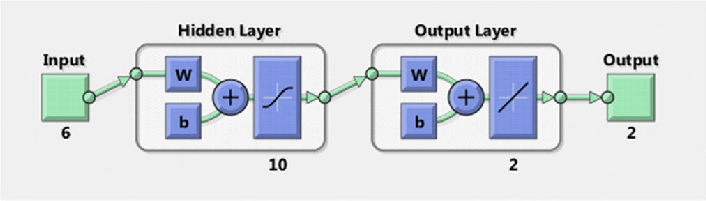
\includegraphics[scale=1]{Images/nftool.png}
	\caption{NN standard architecture}
	\label{fig:nftoolarch}
\end{figure}

In the following subsections the factors influencing the training will be described. Throughout the refinement phase, they have been tuned in order to reach progressively better performance.

%------------------------------------------------

\subsection{Input \& Output}

As previously mentioned, Table \ref{table:inputprm} lists the parameters used as inputs for the NN. 
Knowing the ranges in which the desired parameters could sweep, different randomized sets of output values have been used as network output targets. 
The corresponding input vectors \textit{$ \omega $(t)} and \textit{i(t)} data have been calculated from their respective transfer functions

\begin{equation}
	\omega = \dfrac{K}{s^2J_mL+}
\end{equation} 

%------------------------------------------------

\subsection{Subsection 3.2}

Text

%------------------------------------------------

\subsection{Subsection 3.3}

Text

\pagebreak

%----------------------------------------------------------------------------------------
%	REFERENCES
%----------------------------------------------------------------------------------------


\section*{\textbf{References}}

\begin{enumerate}
	\item Wikipedia - \textit{Class Action} (movie)
	\item Wikipedia - Punitive Damages
	\item Dana P. Babb - "The Deployment of Car Manufacturers into a Sea of Product Liability? Recharacterizing Preemption as a Federal Regulatory Compliance Defense in Airbag Litigation", Washington University Law Review - Volume 75 | Issue 4, 1997.
	\item Mark Dowie - "Pinto Madness", Mother Jones, 1997.
	\item Robert Sherefkin - "Lee Iacocca's Pinto: A fiery failure", Automotive News, 2003.
	\item Wikipedia - Grimshaw v. Ford Motor Co.
\end{enumerate}

\end{document}